%worksheet3.tex
%problem set for the course PandA2 COMS10001 taught at the University of Bristol
%2017 Conor Houghton conor.houghton@bristol.ac.uk

%To the extent possible under law, the author has dedicated all copyright 
%and related and neighboring rights to these notes to the public domain 
%worldwide. These notes are distributed without any warranty. 



\documentclass[11pt,a4paper]{scrartcl}
\typearea{12}
\usepackage{graphicx}
\usepackage{pstricks}
\usepackage{tikz-qtree}
\usepackage{listings}
\usepackage{color}

\newif\ifanswers
\answerstrue
%\answersfalse


\lstset{language=C}
\pagestyle{headings}
\markright{COMS10001 - PandA2 algorithms worksheet 3 - Conor}
\begin{document}

\subsection*{Algorithms Worksheet 3}

This week there is only one question worth eight marks, there are two
marks for attendance.

\begin{enumerate}

\item Draw the tree for the $(3,1,1)$ game of nim and use minimax to decide which move the first player should play.
\end{enumerate}

\ifanswers

\noindent Solution:
So first of all we draw the tree, unbold marks the first player.
\begin{center}
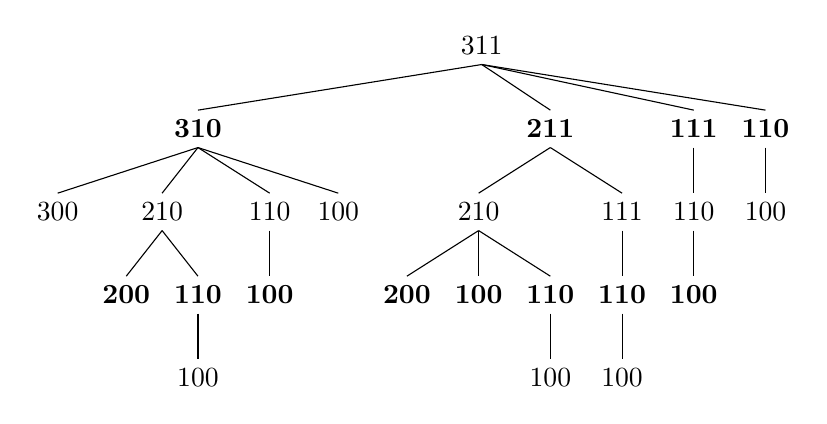
\begin{tikzpicture}
\Tree
    [.311 
      [.\textbf{310}
        [.300 ]
        [.210
          [.\textbf{200} ]
          [.\textbf{110} 100 ]
        ]
        [.110 \textbf{100} ]
        [.100 ]
      ]
      [.\textbf{211} 
        [.210
          [.\textbf{200} ]
          [.\textbf{100} ]
          [.\textbf{110} 100 ]
        ]
        [.111
          [.\textbf{110} 100 ]
        ]
      ]
      [.\textbf{111} 
        [.110 \textbf{100} ]
      ]
      [.\textbf{110} 100 ]
    ]
\end{tikzpicture}
\end{center}
Now, mark the wins for unbold at +1 and for bold as -1.
\begin{center}
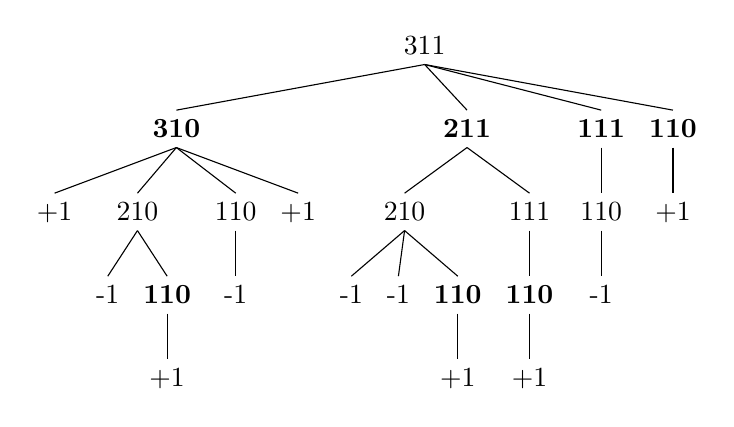
\begin{tikzpicture}
\Tree
    [.311 
      [.\textbf{310}
        [.+1 ]
        [.210
          [.-1 ]
          [.\textbf{110} +1 ]
        ]
        [.110 -1 ]
        [.+1 ]
      ]
      [.\textbf{211} 
        [.210
          [.-1 ]
          [.-1 ]
          [.\textbf{110} +1 ]
        ]
        [.111
          [.\textbf{110} +1 ]
        ]
      ]
      [.\textbf{111} 
        [.110 -1 ]
      ]
      [.\textbf{110} +1 ]
    ]
\end{tikzpicture}
\end{center}
and now we propagate those scores upwards, assuming unbold choses the +1 and -1 the -1.
\begin{center}
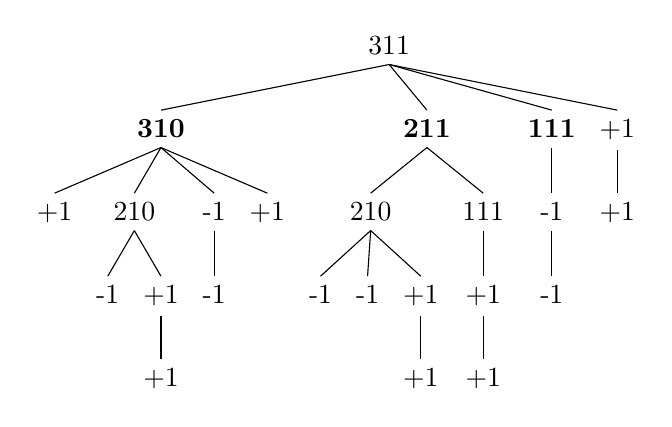
\begin{tikzpicture}
\Tree
    [.311 
      [.\textbf{310}
        [.+1 ]
        [.210
          [.-1 ]
          [.+1 +1 ]
        ]
        [.-1 -1 ]
        [.+1 ]
      ]
      [.\textbf{211} 
        [.210
          [.-1 ]
          [.-1 ]
          [.+1 +1 ]
        ]
        [.111
          [.+1 +1 ]
        ]
      ]
      [.\textbf{111} 
        [.-1 -1 ]
      ]
      [.+1 +1 ]
    ]
\end{tikzpicture}
\end{center}
and

\begin{center}
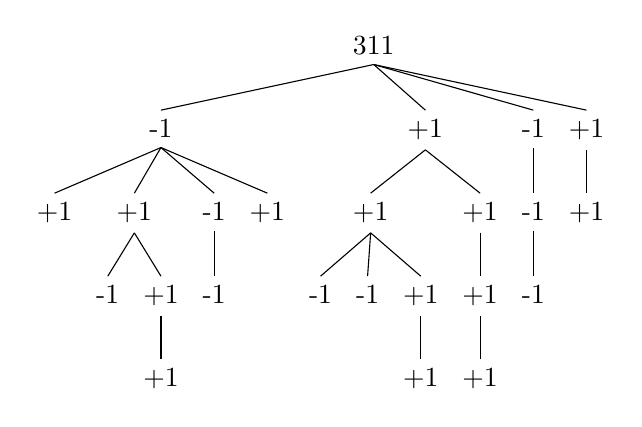
\begin{tikzpicture}
\Tree
    [.311 
      [.-1
        [.+1 ]
        [.+1
          [.-1 ]
          [.+1 +1 ]
        ]
        [.-1 -1 ]
        [.+1 ]
      ]
      [.+1 
        [.+1
          [.-1 ]
          [.-1 ]
          [.+1 +1 ]
        ]
        [.+1
          [.+1 +1 ]
        ]
      ]
      [.-1 
        [.-1 -1 ]
      ]
      [.+1 +1 ]
    ]
\end{tikzpicture}
\end{center}
so the first player can win if they go to $(2,1,1)$ or $(1,1,0)$.
\fi

\end{document}
